\chapter{Implementation}
\label{chap:opendial}
\index{openDial@\opendial{}|textbf}

This chapter outlines the architecture and most important features of the \opendial{} toolkit.\footnote{The name of the toolkit was chosen because of the open design that characterises the framework, and more particularly its extensible, domain-independent architecture with a declarative domain specification.} \opendial{} is a Java-based software toolkit developed to construct and evaluate dialogue systems based on probabilistic rules. The toolkit aims to be fully generic and domain-independent, since all domain-specific knowledge is captured in the declarative specification\index{dialogue domain!declarative design of} of the dialogue domain.

The toolkit implements all the data structures and algorithms detailed in this thesis and served as our experimental platform to carry out the empirical studies presented in Chapters \ref{chap:wozlearning}, \ref{chap:rllearning} and \ref{chap:user-evaluation}. Dedicated components have been developed to interface \opendial{} with the Nao robotic platform and adapt the architecture to human--robot interaction settings.

The chapter is divided in two sections.  The first section focuses on the design of the \opendial{} toolkit and describes its general workflow, the specification of dialogue domains in XML, and the concrete implementation of the algorithms employed for approximate inference, sampling and forward planning. We also briefly compare the toolkit to other types of dialogue architectures and discuss its current technical limitations.  The second section goes on to explain how the toolkit is integrated and extended into a full-fledged dialogue system for human--robot interaction, describing both the general system structure as well as the individual components developed to control the verbal and non-verbal behaviour of the robot.  

\section{Toolkit design}
\label{sec:genarchitecture}

\subsection{Generalities}

The \opendial{} toolkit relies on an event-driven blackboard architecture\index{blackboard architecture}. Blackboard architectures are widely used in spoken dialogue systems for their ability to handle flexible workflows where multiple modules ``cooperate'' to  interpret the user inputs, maintain a representation of the dialogue state, and decide on the action(s) to perform. In spoken dialogue systems, the blackboard corresponds to the system state, while the modules attached to this blackboard are in charge of specific processing tasks such as speech recognition and understanding, dialogue management, natural language generation and speech synthesis. 

%information state approaches are notably based on such architecture. 

\subsubsection*{System scheduling}

The modules read and write to the dialogue state in an event-driven manner\index{event-driven architecture} . After each change, the dialogue state sends an event message to all its attached modules to inform them of the state update. When appropriate, the modules can react to such events and further modify the dialogue state, thereby generating new updates. The process continues until the dialogue state is stabilised.\footnote{Recall that a model can only be applied once per update to avoid infinite cycles (cf. Algorithm \ref{algo:stateupdate}).}   The \opendial{} toolkit allows system modules\index{system modules} to run in parallel via multi-threading. The possibility to execute modules in parallel is particularly useful in dialogue systems, as the agent must be able to react to new inputs and contextual changes occurring at any time -- even while other modules are still busy processing a previous update.  Many of the algorithms developed in the toolkit -- such the ones used for planning and probabilistic inference -- also operate in anytime mode, which implies that they can be gracefully interrupted and deliver their outputs at any time.

At the time of writing, the implementation of \opendial{} is optimised to run on a single platform.\footnote{System modules can, however, remotely connect to external resources on the robotic platform to perform tasks related to robot perception and motor control, as explained in Section \ref{sec:system-integration}.} Should such a need arise, the framework could be extended to run on multiple platforms, as the blackboard paradigm generally lends itself well to distributed architectures\index{distributed architecture} \citep{Corkill:1989}.

\subsubsection*{Components}

The modules connected to the dialogue state in the \opendial{} toolkit can be divided into two categories. The first type of module is the rule-structured model\index{rule-structured model} already outlined in Section \ref{sec:processing-workflow}.  A rule-structured model is simply defined as a collection of probabilistic rules together with a list of trigger variables.  The update of (at least) one of these trigger variables in the dialogue state results in the instantiation of the probabilistic rules in the dialogue state. In addition to these rule-structured models, the \opendial{} toolkit also includes external components such as the speech recogniser, text-to-speech engine and processes for robot perception and control. Given the blackboard architecture of the toolkit, modules can be easily plugged in and out of the system without affecting the rest of the processing pipeline. Similarly to the rule-structured models, external components operate by monitoring the dialogue state and updating it when relevant changes are detected. 

In the experiments carried out in this thesis, we found it useful to encode not only dialogue management models with the help of probabilistic rules, but also tasks related to natural language understanding and generation. As argued in \cite{lison-semdial2012}, the expressive power of probabilistic rules allows them to capture the structure of many dialogue processing tasks, not necessarily confined to dialogue management. However, the parameters of the NLU and NLG models are hand-crafted since they do not directly constitute the focus of our work. 

%The dialogue domain designed for the experiment conducted in the next chapter includes for instance a total of six models: one dialogue act classification model, (triggered by the user utterance $u_u$), one utility model (triggered by the user dialogue act $a_u$), three probability models to predict the effects of the system action on the context, the user intention and the next user action (all triggered by the system action $a_m$), and a generation model (triggered by the system action $a_m$). 

Compared to traditional architectures in which the components are developed separately and rely on ad hoc representation formats, the use of a shared description formalism (probabilistic rules) to encode multiple reasoning tasks offers several advantages:
\begin{itemize}
\item \textit{Transparency}\index{system transparency}:  The reliance on a common representation format provides a unified, transparent semantics for the dialogue state, since all state variables are described and related to one another through a principled framework grounded in probabilistic modelling.  This makes it possible to derive a semantic interpretation for the dialogue state as a whole, in terms of a joint probability distribution over the state variables. 

\item \textit{Domain portability}\index{system portability}:   As most domain-specific knowledge is declaratively specified in the rules, the system architecture is essentially reduced to a generic platform for rule instantiation and probabilistic inference.  This declarative design greatly enhances the system portability across domains, since adapting a system to a new domain only requires a rewrite or extension of the domain-specific rules, without having to reconfigure or re-develop other components.  This stands in sharp contrast with ``black-box'' types of architectures\index{black-box architecture} where much of the task- and domain-specific knowledge is encoded in procedural form buried inside the implementation of the system components.

\item \textit{Flexible workflow}\index{system workflow}:  Probabilistic rules allow for very flexible processing pipelines where state variables are allowed to depend or influence each other in any order and direction.  New rule-structured models can be easily inserted or extended without requiring any change to the underlying platform. Furthermore, several models can be triggered concurrently on the same input/output variables. As we have seen in Section \ref{sec:probruleinstantiation}, output distributions can indeed depend on an arbitrary number of rule nodes and handle effects arising from multiple, sometimes conflicting sources. This allows the system to take advantage of multiple, complementary processing strategies while ensuring that the representation of the dialogue state as a whole remains consistent. 

\item \textit{Joint optimisation}\index{joint optimisation}:  Finally, the use of a unified formalism allows domain models to be optimised jointly instead of being tuned in isolation from one another. Joint optimisation has recently gained much attention in the dialogue systems community to overcome the fragmentation of current system architectures and attempt to directly optimise the end-to-end conversational behaviour of the system \citep[see also][]{Lemon:2011}. 

\end{itemize}

Despite these merits, probabilistic rules cannot naturally model all dialogue reasoning tasks.  Modules such as speech recognition or speech synthesis depend in particular on external resources and processes and must be integrated separately in the system. The \opendial{} toolkit is designed to incorporate both rule-structured models and external components in its architecture. 
\subsection{Specification of dialogue domains}
\label{sec:domain-specification}

\subsubsection*{Dialogue domains}
\index{dialogue domain}
As already mentioned in Section \ref{sec:processing-workflow}, a dialogue domain is represented in \opendial{} by a pair $\langle \mathcal{B}_0, \mathcal{M} \rangle$ defined by an initial dialogue state $\mathcal{B}_0$ and a set of models $\mathcal{M}$, each model being itself composed of a collection of probability or utility rules. Dialogue domains are encoded in an XML\index{XML} format\footnote{XML (Extensible Markup Language) is a general-purpose markup language for encoding and exchanging documents, as specified by the World Wide Web Consortium (W3C), cf. \urlsmall{http://w3.org/xml}.} with a syntax specifically designed for the toolkit. 

In practice, the specification of a dialogue domain in XML takes the following form: \vspace{2mm}
\lstset{language=XML}
\begin{lstlisting}
        <domain> &\vspace{2mm}&
            <initialstate>    
                <!-- initial state variable values -->
            </initialstate>

            <model trigger="trigger variable(s) for model 1">
                <!-- rules for model 1 -->
            </model>  &\vspace{2mm}& 
            ... &\vspace{2mm}&
            <model trigger="trigger variable(s) for model n">
                <!-- rules for model n -->
     	    </model>&\vspace{2mm}&
        </domain>
\end{lstlisting}\vspace{2mm}

The initial dialogue state is represented as a list of state variables, each being associated with a particular probability distribution.  Most state variables are defined by a categorical distribution, according to the following skeleton:\index{categorical distribution}

\vspace{3mm}\begin{lstlisting}
        <variable id="variable name">
            <value prob="probability for first value">&\color{black}{first value}&</value>
            <value prob="probability for second value">&\color{black}{second value}&</value>
            ...
            <value prob="probability for nth value">&\color{black}{nth value}&</value>
       </variable>  
\end{lstlisting}\vspace{2mm}

State variables defined over continuous ranges can also be encoded with probability density functions. In such a case, the state variable is defined by a particular distribution family and a specification of parameters associated with that family. 

\subsubsection*{Probabilistic rules}
\index{probabilistic rule}\index{probability rule}

Each model specification encompasses a number of probability or utility rules also encoded in XML. Listing \ref{listing:xml1} illustrates an example of an XML specification for a probability rule. The rule expresses the probability of the user intention $\mathit{Release}(X)$, which corresponds to the action of putting down a carried object $X$ onto the ground.  The probability of this user intention is naturally dependent on the completion status of the previous task and on whether the object $X$ is currently carried by the robot. The values of the Dirichlet parameters $\boldsymbol\theta_{\text{release1}}$ and $\boldsymbol\theta_{\text{release2}}$ are unknown, but we may presuppose that the user intention $i_u = \mathit{Release}(X)$ is much more likely whenever the robot actually carries the object $X$. 

Each rule is divided in a number of cases, each containing a (possibly empty) condition and a set of (possibly empty) effects.  Conditions can include several sub-conditions combined by conjunction or disjunction operators (the default operator being a conjunction). Each basic condition is denoted by an ``\begin{small}\textsf{if}\end{small}'' markup and is composed of three elements: a variable label, a value, and a binary relation that must hold between the variable and the value. The default relation is equality, but relations may also correspond to inequalities ($\neq$, $<$ and $>$), set inclusion ($\in$ and $\notin$) or string matching operations.   More complex logical constructions with nested conjunctions, disjunctions and negation operators can be accounted for via additional XML markup (not shown in the example). 

Effects are associated with probabilities that can either be fixed or correspond to parameters to learn such as the Dirichlet distributions $\boldsymbol\theta_{\text{release1}}$ and $\boldsymbol\theta_{\text{release2}}$ in the example.  Although the effects in the example only have one single output variable, rules are allowed to include multiple ``\begin{small}\textsf{set}\end{small}'' markups to express complex effects ranging over more than one output variable. Universally quantified variables such as $X$ are wrapped in curly brackets \{ \} to distinguish them from the rest of the text. These variables can occur in both the conditions and effects of the rule. 

Utility rules\index{utility rule} are defined in the same manner.  An example of a utility rule specified in XML is given in Listing \ref{listing:xml2}.  The rule defines the utility of asking the user to confirm the last system action $\mathit{Demonstrate}(X)$ after a certain amount of silence, divided here in three cases (between one and two seconds, between two and three seconds, and after three seconds).  Three utility parameters $\theta_{\text{confirm1}}$ $\theta_{\text{confirm2}}$ and $\theta_{\text{confirm3}}$ are associated with the utility rule.  A universally quantified variable $X$ is also employed here to generalise the rule to arbitrary arguments for the system action $a_m = \mathit{Demonstrate}(X)$. 

\begin{lstlisting}[label=listing:xml1,caption=Example of probability rule in XML format., float=p,captionpos=b]
            <rule>
                <quantifier id="X"/>
                <case>
                    <condition>
                        <if var="completed-task" value="true" />
                        <if var="carried" value="{X}" relation="contains" />
                    </condition>
                    <effect prob="theta_release1[0]">
                        <set var="i_u" value="Release({X})" />
                    </effect>
                    <effect prob="theta_release1[1]" />
                </case>
                <case>
                    <condition>
                        <if var="completed-task" value="true" />
                    </condition>
                    <effect prob="theta_release2[0]">
                        <set var="i_u" value="Release({X})" />
                    </effect>
                    <effect prob="theta_release2[1]" />
                </case>
            </rule>
\end{lstlisting}


\begin{lstlisting}[label=listing:xml2,caption=Example of utility rule in XML format., float=p,captionpos=b]
            <rule>
                <quantifier id="X"/>
                <case>
                    <condition>
                        <if var="silence" value="3" relation=">"/>
                        <if var="a_m" value="Demonstrate({X})"/>
                    </condition>
                    <effect utility="theta_confirm1">
                        <set var="a_m" value="AskConfirmation"/>
                    </effect>
                </case>
                <case>
                    <condition>
                        <if var="silence" value="2" relation=">"/>
                        <if var="a_m" value="Demonstrate({X})"/>
                    </condition>
                    <effect utility="theta_confirm2">
                        <set var="a_m" value="AskConfirmation"/>
                    </effect>
                </case>
                <case>
                    <condition>
                        <if var="silence" value="1" relation=">"/>
                        <if var="a_m" value="Demonstrate({X})"/>
                    </condition>
                    <effect utility="theta_confirm2">
                        <set var="a_m" value="AskConfirmation"/>
                    </effect>
                </case>
            </rule>
\end{lstlisting}

\subsubsection*{Parameters}

When operating in learning mode, dialogue domains must be associated with parameter variables defined together with their prior probability distribution.  This prior can take the form of a categorical, Dirichlet, Gaussian or uniform distribution.  As an illustration, the prior distribution for the parameter variable $\boldsymbol\theta_{\text{release1}} \sim \mathrm{Dirichlet}(1,2)$ is specified as: 

\vspace{3mm}\begin{lstlisting}
        <variable id="theta_release1">
            <distrib type="dirichlet">
                <alpha>&\color{black}{1}&</alpha>
                <alpha>&\color{black}{2}&</alpha>
            </distrib>
        </variable>
\end{lstlisting}\vspace{2mm}

Other types of prior distributions are defined in a similar manner. 

\subsection{Core algorithms}
\label{sec:corealgorithms}

We survey below a number of technical aspects related to the \opendial{} implementation of the core algorithms presented through this thesis.  

\subsubsection*{Inference}
\index{probabilistic inference}

Probabilistic inference forms a key element in the state update process.  Two distinct types of inference algorithms are implemented in \opendial{}: \begin{enumerate}
\item The first is variable elimination\index{variable elimination}, which is an exact inference method initially developed by \cite{ZhangP96}.  The algorithm operates by manipulating matrices through summation and pointwise products. The particular implementation of this algorithm in \opendial{} follows the method presented in \cite[][p. 1101]{Koller+Friedman:09}, which generalises classical variable elimination to decision networks.
\item The second inference algorithm is likelihood weighting\index{likelihood weighting}, which is an approximate inference method relying on importance sampling. As explained in Section \ref{sec:inference}, likelihood weighting generates samples based on the topological ordering of the graphical model. Each sample is associated with a particular weight that represents its likelihood in the light of the provided evidence.  The final estimates correspond to the weighted averages of the samples. 
\end{enumerate}

Each inference algorithm has its own strengths and weaknesses. Variable elimination is able to deliver provably exact results and is often the most efficient inference method for small graphical models.  However, variable elimination suffers from scalability problems when applied to models that are densely interconnected and/or include continuous variables. Likelihood weighting is easier to scale to larger networks and can be straightforwardly applied to hybrid models with both discrete and continuous variables. However, large numbers of samples are required to reach reasonably accurate estimates.

In order to bring together the best of both approaches, a switching mechanism has been integrated to \opendial{} to automatically select the inference method that is best suited to each probabilistic query.  The mechanism proceeds as follows. For each probabilistic query, three elements are extracted: the maximum branching factor of the network, the number of continuous variables, and the number of variables specified in the query. These elements are then matched against predefined thresholds. If at least one threshold is exceeded, likelihood weighting is selected to perform the inference, while variable elimination is chosen in the remaining cases. 

\subsubsection*{Sampling techniques}
\index{sampling techniques}

The use of likelihood weighting necessitates the implementation of efficient sampling techniques for each possible probability distribution.  We describe below the sampling methods employed in \opendial{} to efficiently draw values from both discrete and continuous distributions:
\begin{itemize}
\item \textit{Categorical distributions}\index{categorical distribution}:  Sampling a categorical distribution is done through inverse random sampling, following the method described in \citet[p.~489]{Koller+Friedman:09}. When constructing the distribution, the variable values are sorted according to lexicographic order, and a cumulative density function (CDF) calculated relative to this order.  Sample values are then extracted at runtime by (1) generating a pseudo-random float number between 0 and 1 and (2) locating the greatest number in the CDF that is less than or equal to the number just generated.  Operation (2) is done via binary search. The value indexed by this number is then selected as the sample.
\item \textit{Uniform distributions}\index{uniform distribution}:  Uniform distributions are directly sampled as $g (b-a) + a$, where $g$ is a pseudo-random number between 0 and 1, and $a,b$ are the distribution boundaries.

\item \textit{Normal distributions}\index{normal distribution}:  Normal distributions are sampled in \opendial{} via the well-known Box-Muller method \citep{rBOX58a}, which derives two sample values for a given normal distribution based on two pseudo-random numbers.

\item \textit{Dirichlet distributions}\index{Dirichlet distribution}:  Sampling Dirichlet distributions relies on a slightly more intricate procedure based on Gamma sampling.   The first step is to derive $K$ samples from $\mathrm{Gamma} (\alpha_i, 1)$ with $K$ denoting the dimension of the Dirichlet and $1 \leq i \leq K$.  This sampling procedure is implemented in \opendial{} using the method presented in \cite{cheng1979}.  The sampled Dirichlet value is then defined as $[x_1,...x_K]$ where $x_i = \frac{y_i}{\sum_{j=1}^K y_j}$ and $y_i$ is the sampled Gamma value for dimension $i$.
\item \textit{Kernel distributions}\index{kernel density estimation}:  We sample non-parametric distributions defined via kernel density estimation (KDE) in two steps. The first is to draw at random one point $x_i$ from the set of points $x_1,...x_n$ included in the KDE. A value is then drawn from the kernel associated with the point. In our case, this corresponds to drawing a sample from the normal distribution $\mathcal{N}(x_i,h)$ centred at $x_i$ and of variance $h$ (the bandwidth). 
\end{itemize}

\subsubsection*{Online planning}
\index{online planning}
The implementation of the forward planning algorithm closely follows the procedure outlined in Section \ref{sec:modelbased}.  The search tree is constructed in a breadth-first manner, until either the planning horizon has been reached or the planner has run out of time.  The latter condition relies on a time-out function to ensure that the planner does not exceed specific time limits.

In order to generate a set of possible observations in a given state $\mathcal{B}$ (line 6 of Algorithm \ref{algo:planning}), the planner locates all predictive state variables (denoted with a superscript $p$) currently present in the dialogue state and draws a sample value for each.  In the experiment presented in Section \ref{sec:rllearning-experiments}, the predictive variable corresponds to the next user action, and the generated observations will therefore reflect possible values for this user action.

For tractability reasons, \opendial{} limits the maximum number of actions and observations that are branched out at each point in the search tree.  The actions are selected on the basis of their reward values in the current state -- i.e.\ only the $n$ actions with highest reward are selected, with $n$ corresponding to an arbitrary threshold. The observations are filtered based on their likelihood of occurrence.  The planner thus only expands the tree with the $m$ most likely observations, where $m$ is another threshold. The two thresholds are currently manually tuned, but could in principle correspond to additional parameters to optimise during learning. 

\subsection{Comparison with other architectures}
\label{sec:archi-comparison}
\index{dialogue system architecture}

The construction of generic, domain-independent architectures is a recurring theme in dialogue systems research, and there is a clear trend towards the development of platforms composed of more generic or reusable components. We present below the most important architectures currently deployed and contrast their design with the one followed in the \opendial{} toolkit. Finally, we discuss the current limitations of the presented framework.

\subsubsection*{Existing software frameworks}

Information state\index{information state} approaches are closely related to the framework presented in this thesis. The TrindiKit\index{TrindiKit} architecture presented by \cite{Larsson:2000} relies on a shared information state accessed by various system modules and a rich repository of rules. A control module is in charge of the system scheduling for the whole architecture. The system modules can also connect to external resources such as databases and plan libraries.   The TrindiKit is a platform for constructing and evaluating dialogue engines and is designed to be fully domain-independent. The related DIPPER architecture described in \cite{Bos2003} is built on similar principles as the TrindiKit, but simplifies the architecture and the encoding format for the  update rules.  DIPPER\index{DIPPER} employs the Open Agent Architecture as its communication protocol.

The idea of domain independence is also taken up by plan-based approaches such as TRIPS\index{TRIPS} \citep[The Rochester Interactive Planning System, cf. ][]{Allen:2000:AGD:973935.973937}. TRIPS uses an agent-oriented architecture comprising multiple modules working together to recognise the intentions of the human user and fulfilling the system goals.  Most reasoning tasks are explicitly cast as planning problems, from high-level planning to response planning and surface realisation.  

One of the most mature platforms for prototyping dialogue systems is Olympus\index{Olympus/Ravenclaw} and its associated dialogue management framework, called Ravenclaw \citep{Bohus:2007,Bohus:2009}.  The Olympus architecture is built on top of a centralised message-passing infrastructure in which modules can be plugged in and out to suit the needs of the application.  Ravenclaw is a plan-based, task-independent dialogue engine which is fully integrated in Olympus.  Ravenclaw supports mixed-initiative interaction and integrates dedicated functions for error handling, timing and turn-taking. Action selection is based on a hierarchical decomposition of tasks whose execution is sequentially ordered using an agenda structure. 

The agent-based Jaspis\index{Jaspis} architecture \citep{jaspis2004} also has multiple points of contact with the \opendial{} toolkit, as it similarly revolves around a shared representation of the system state.  Jaspis components are themselves split into agents (in charge of decision-making), evaluators (in charge of selecting the most suitable agent in a particular situation) and managers (in charge of the general coordination of the components). Jaspis is designed to allow for distributed setups with dedicated mechanisms for the coordination and synchronisation of concurrent modules.  The architecture also aims to facilitate system-level adaptivity.  Compared to the \opendial{} toolkit, Jaspis offers more advanced support for distributed and parallel setups, but at the cost of an increased system complexity.  

Most MDP\index{dialogue management!MDP approaches to} and POMDP-based dialogue\index{dialogue management!POMDP approaches to} architectures line up system components in a single processing sequence. The prototype systems developed for the TALK and CLASSIC projects \citep{Henderson:2008,Lemon:2012} and the related BUDS POMDP system\footnote{Bayesian Update of Dialogue State, cf. \begin{scriptsize}\url{http://mi.eng.cam.ac.uk/~mh521/nipsdemo12/}\end{scriptsize}} are structured into pipelines where each component takes a probability distribution over input hypotheses and generates another distribution over possible outputs.  

%Contrary to the logic-based architectures mentioned above, these approaches explicitly account for state uncertainty and allow for automatic optimisation of dialogue policies. 


\subsubsection*{Comparison and discussion}

The \opendial{} toolkit can be seen as an attempt to combine the flexibility of information state architectures with the robustness and adaptivity of statistically optimised dialogue systems.  In line with logic-based approaches (e.g.\ TrindiKit, DIPPER, TRIPS, Olympus/Ravenclaw, and Jaspis), the workflow of \opendial{} is designed to allow for multiple processing paths and context-sensitive reasoning strategies.  And in line with MDP and POMDP-based approaches, the toolkit is also able to explicitly handle uncertain knowledge and stochastic relations between variables thanks to its probabilistic representation of the system state, as well as its ability to optimise domain models from interaction data via statistical inference.  

The idea of combining statistical and symbolic approaches to dialogue processing is certainly not novel in the literature on spoken dialogue systems.  In many of the aforementioned dialogue architectures, probabilistic reasoning techniques already coexist with classical symbolic components operating with deterministic inputs. Very often, this integration of heterogeneous statistical and symbolic components is achieved by reducing N-best lists to their single most likely hypothesis. However, an important drawback of such an approach is the substantial loss of information that results from this reduction. For instance, speech recognition typically provides explicit measures of uncertainty in the form of e.g.\ confidence scores, but these confidence measures are often lost at higher reasoning stages such as syntactic parsing, semantic interpretation and dialogue management. 

One can also observe some design differences in the representation of the action selection process. Many dialogue architectures indeed decompose dialogue management into two or more distinct behavioural layers.  The Olympus framework incorporates for instance both an interaction manager in charge of the low-level control of the conversational floor, and a dialogue manager in charge of higher-level dialogue decisions.  The TRIPS architecture similarly divides dialogue management in a cluster of modules encompassing discourse management, discourse context management, plan management, and a behavioural agent in charge of controlling the overall behaviour. The \opendial{} toolkit leaves by comparison the system designer free to frame decision-making in one, two or more layers, depending on the particular needs of the domain.\footnote{This can be practically realised by creating distinct utility models for action selection.  Hierarchical decision policies can notably be captured by lining up utility models in a top-down cascade of triggers.} 

The declarative specification of the dialogue domain in terms of rule-structured models facilitates a modular design of the system's internal knowledge base.  The formalism of probabilistic rules is sufficiently general to encode a broad range of dialogue models, from highly domain-specific constraints and heuristics to more generic conversational skills. However, in contrast to frameworks such as Olympus/Ravenclaw, \opendial{} leaves the distinction between domain-specific and domain-independent models entirely into the hands of the system designer and does not enforce a particular decomposition between these two types of system knowledge  at the architectural level. Similarly, \opendial{} does not commit to a particular encoding of the common ground or to a specific grounding strategy.  However, the expressive power of probabilistic rules (and their support of logical operators) allows them to capture rich representations of the interaction dynamics -- including grounding phenomena -- and their effects on the dialogue state. 


%Many dialogue architectures have been specifically engineered to handle situated or multimodal domains. The WITAS architecture \citep{LemonBGP01} is one of the first dialogue architecture devoted to multimodal settings (in their case an autonomous mobile robot).  The SmartKom system \citep{smartkom} describes the development of another type of multimodal system combining speech, gesture, and mimics.  Our previous work on situated human--robot interaction \citep{cosybook:dialogue} illustrates how dialogue processing can be coupled to sensorimotor components in a bidirectional manner. The Ariadne multimodal dialogue architecture comes especially close to this work due to its use of a declarative specification of the dialogue domain. In a more theoretical realm, the framework of semiotic schemas developed in \cite{Roy05} attempts to bridge the gap between linguistic understanding, action and perception through the use of grounded schemas, with application to interactive robots.  

\subsubsection*{Limitations}

One important aspect of dialogue architectures that has not really been covered in this work is the question of incremental processing\index{incremental processing}.  As explained in the background chapter, dialogue processing should ideally be performed incrementally and output partial hypotheses as early as possible in the system workflow. The InproTK\index{InproTK} architecture presented by \cite{Baumann:2012} and \cite{baumann2013:phd} is specifically designed to support across-the-board incremental processing, from speech recognition to dialogue management and speech synthesis. Although the current implementation of \opendial{} cannot claim to be incremental, we do nevertheless hypothesise that the formalism of probabilistic rules could be extended to allow for incremental processing without major difficulties, since the chain of related hypotheses is already explicitly captured in the conditional dependencies generated by the instantiated rules.  An update in the probability distribution over some observations (e.g.\ the user utterance) is therefore automatically reflected in all hypotheses that depend on it (e.g.\ the corresponding user intention). Modifying the state update algorithm to run in a fully incremental manner without hampering the system performance is, however, a non-trivial engineering task, which could constitute an interesting topic for future work. Similarly, the turn-taking behaviour\index{turn-taking} integrated in \opendial{} remains relatively rudimentary and could certainly be improved to allow for e.g.\ interruptions and fragmented utterances.

While the dialogue system employed for our experiments does include several modules for robot perception and control (cf. next section), the toolkit does not yet support full-scale multi-modal processing\index{multi-modal processing}, as such extensions would require the integration of dedicated mechanisms for information fusion and fission in the architecture. Our own previous work on situated human--robot interaction \citep{cosybook:dialogue} illustrates how dialogue processing can be coupled to sensorimotor components in a bidirectional manner.  

On a more practical note, it should finally be pointed out that \opendial{} is at the time of writing at an early stage of development and does not benefit from the years of incremental refactoring and testing shown by more mature architectures such as TrindiKit or Olympus/Ravenclaw. Further development work is certainly needed to move \opendial{} from being an advanced research prototype to a stable, robust platform capable of being deployed in any application domain. Of special importance is the integration of user-friendly authoring tools\index{domain authoring} to allow human designers to write, organise and evaluate rule-structured dialogue domains without having to delve into the technical intricacies of XML syntax. \opendial{} would also certainly benefit from more advanced performance tuning to enhance the system reactivity and scalability to larger domains. 


%\footnote{In this respect, it is interesting to draw a parallel between dialogue systems and other fields of NLP such as syntactic parsing. Before the sixties, most parsers relied on procedural routines buried in the code.  One of the major advances in parsing has come from the decision to separate the domain knowledge (in this case, the lexicon and grammar) on one hand, and the parsing algorithms on the other hand.  We would argue that dialogue systems could also benefit from a  between declarative knowledge (i.e.\ task- and domain-specific models) and generic processing functionalities (i.e.\ algorithms for reasoning, learning and planning under uncertainty.)}

\section{System integration}
\label{sec:system-integration}
The \opendial{} toolkit was used as a software foundation to construct a concrete, end-to-end dialogue system for human--robot interaction.  We detail in the next pages the practical design of this dialogue system as well as the graphical user interface implemented to monitor and control the system behaviour (and its internal dialogue state) in real-time. 
\index{spoken dialogue systems}
\subsection{Architecture}

In addition to the \opendial{} core components, the dialogue system employed in our experiments also included specific modules for speech recognition and synthesis, robot perception and motor control.  The generic architecture for the system is shown in Figure \ref{fig:impl_architecture}. 

\begin{figure}[ht]
\centering
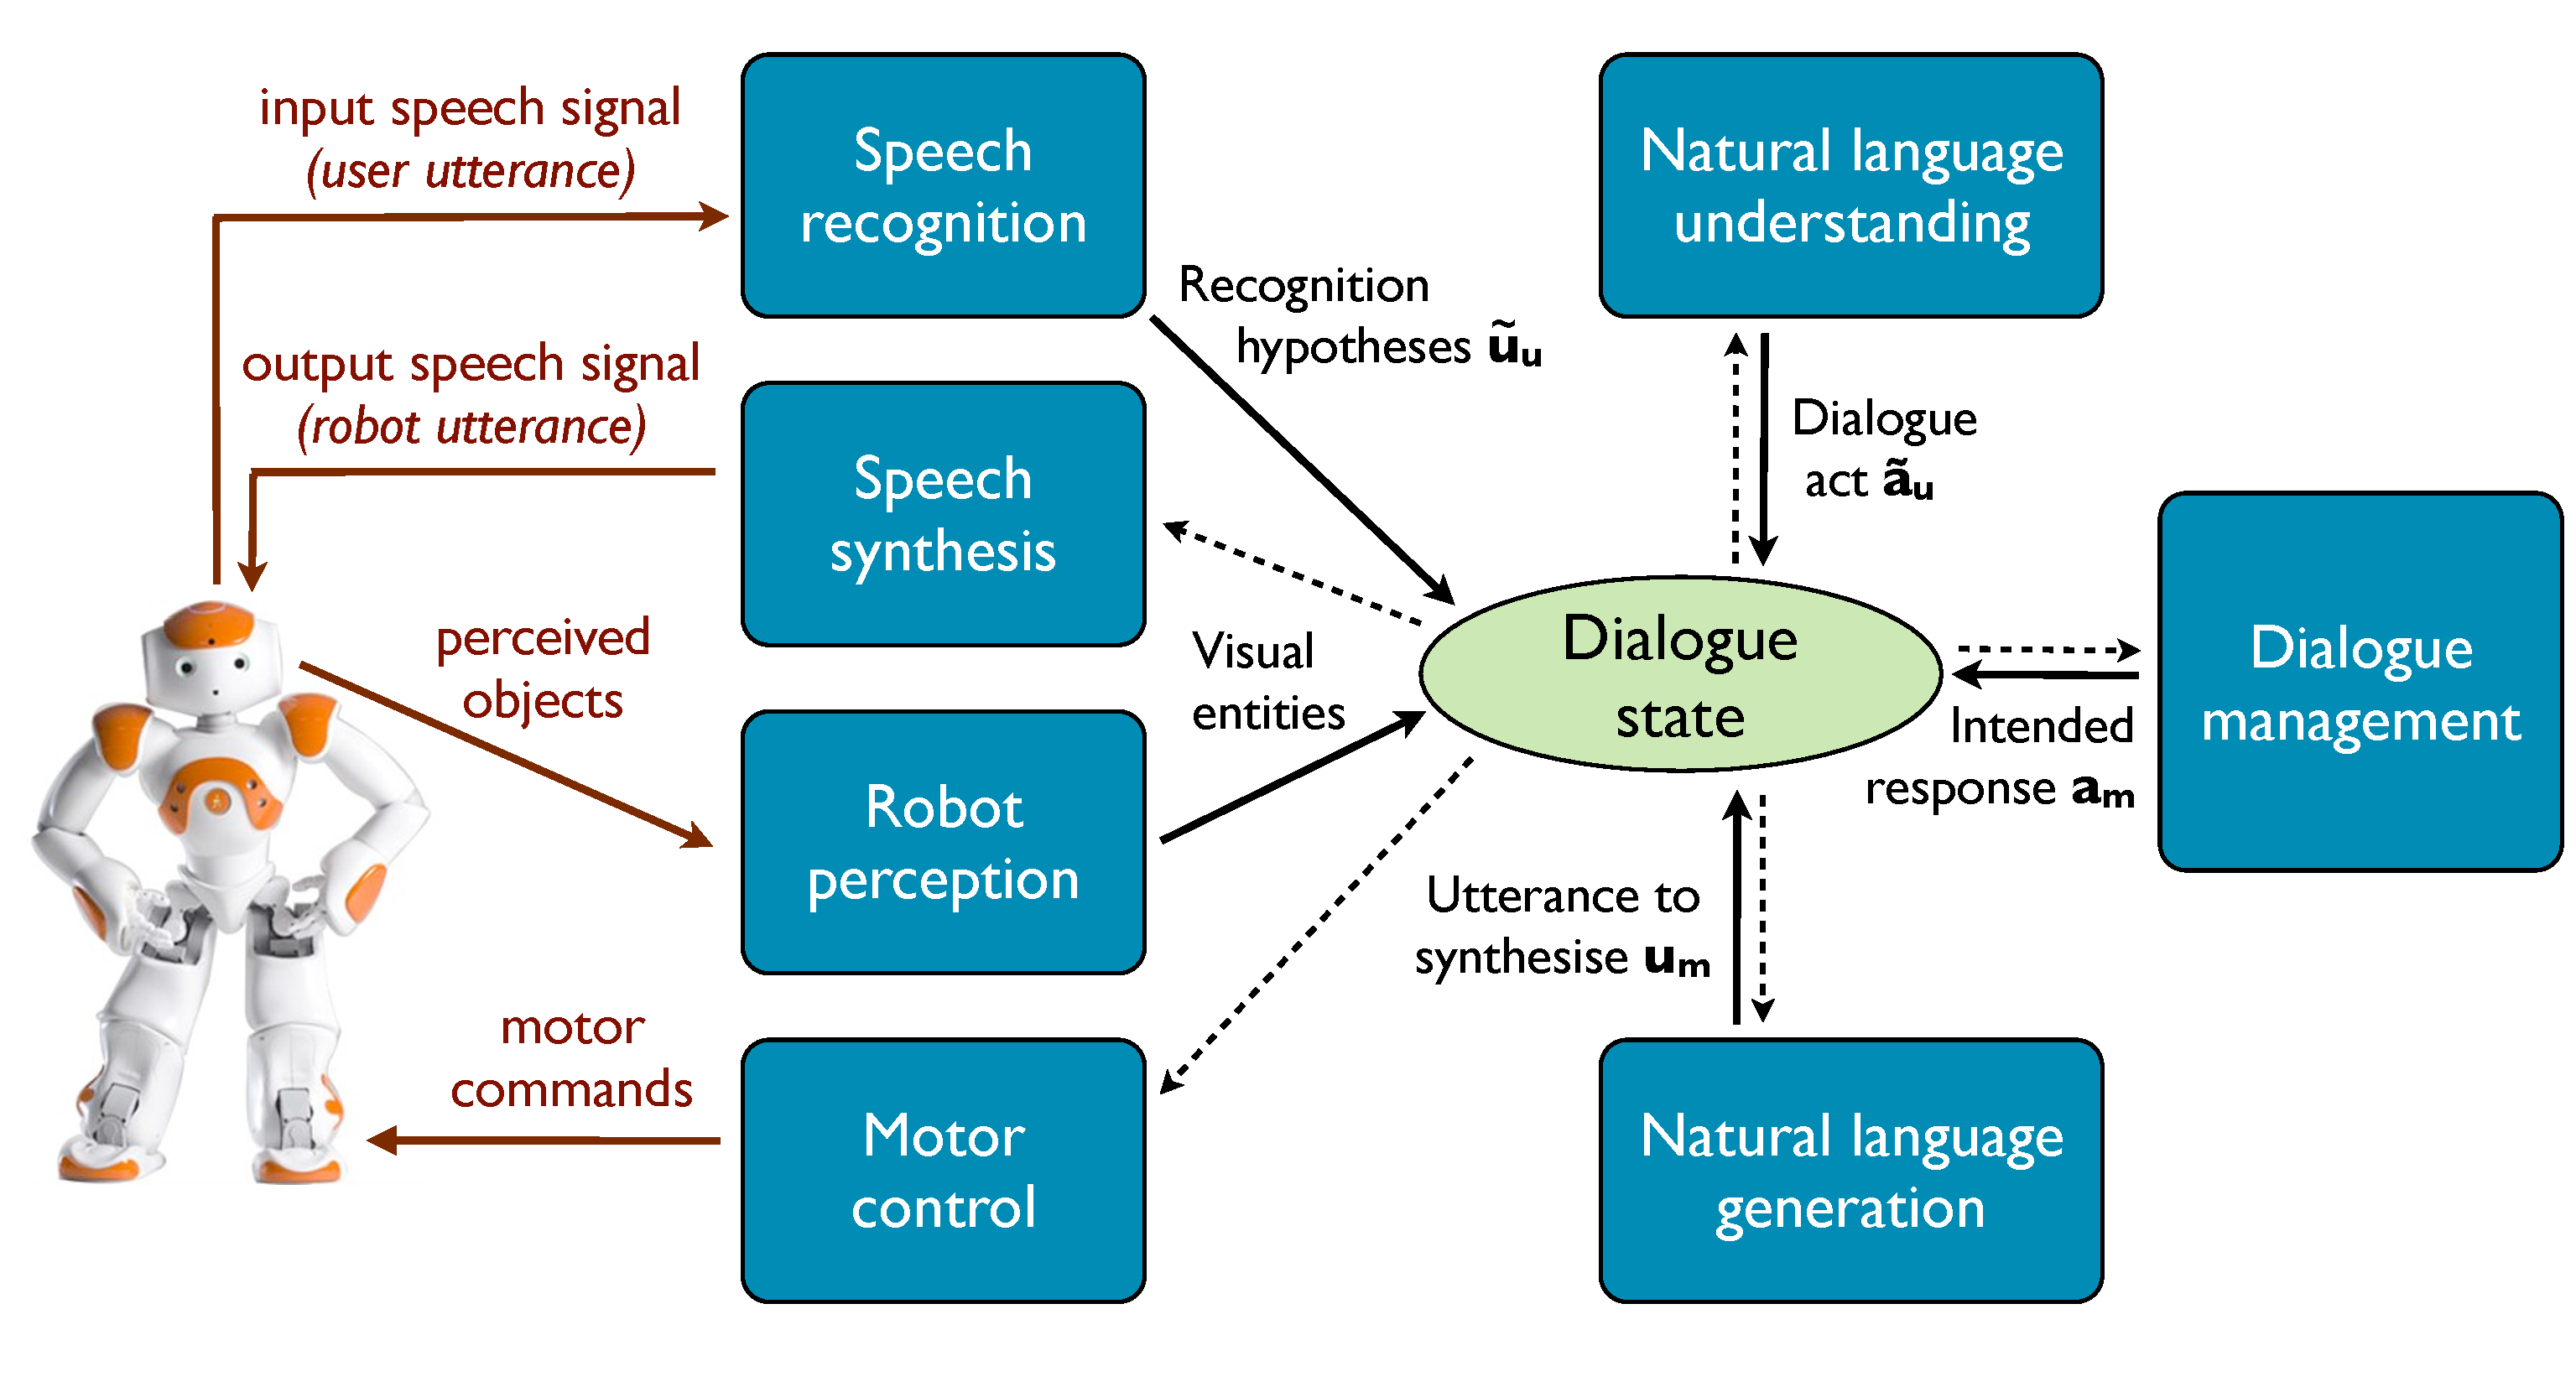
\includegraphics[scale=0.30]{imgs/impl_architecture.pdf}
\caption{Generic system architecture employed in the experiments.}
\label{fig:impl_architecture}
\end{figure}

The system modules can operate in either synchronous or asynchronous mode:\index{synchronous \& asynchronous processing} \begin{itemize}
\item Synchronous modules continuously monitor the dialogue state for relevant changes.  Their activation is thus performed in synchrony with the update events generated by the dialogue state.
\item Asynchronous modules run independently of the dialogue state.  They typically relate to visual or speech perception tasks. Asynchronous modules update the dialogue state as soon as new observations are made available. 

\end{itemize}

All modules have access to the complete dialogue state and can therefore exploit the full set of state variables (including generic contextual information) in their processing. 

\subsection{Individual modules}

We describe below the modules shown in Figure \ref{fig:impl_architecture} and explain their role and internal structure. It should be emphasised that the focus of the present thesis is on dialogue management.  The other system modules are therefore deliberately limited to simple, ``shallow'' processing methods in order to concentrate the implementation efforts on the dialogue manager. %Many of these modules could be extended to employ more sophisticated techniques, in particular in regard to speech recognition, natural language understanding and generation. 

\subsubsection*{Speech recognition}
\index{speech recognition}

Speech recognition is performed on the robot platform, using a commercial, off-the-shelf speech recognition engine (Vocon 3200 from Nuance).  Four microphones placed on the robot head are used for the sound capture.  The placement of the microphones on the robot allows the user to interact with the robot in a natural manner, without needing to resort to head-mounted microphones. This advantage comes, however, at the price of a lower sound quality due to the larger (and varying) distance between the sound source and the microphones.   This distance between source and receiver is indeed a major degradation factor in speech recognition \citep{wolfel2009distant}. Moreover, the microphones are also adjacent to a number of mechanical motors that may disturb the sound signal and lead to spurious detections.

The acoustic model\index{acoustic model} employed in all experiments is based on U.S. English. The language model\index{language model} takes the form of context-free recognition grammars in Bachus-Naur Form. Distinct grammars were used to cover the domain of discourse of each experiment. The grammars were designed by hand, based on the Wizard-of-Oz transcripts collected in our empirical studies (cf. previous chapters). Grammars can be dynamically attached or removed from the engine at runtime, thereby allowing the system to adapt the language model of the recogniser to the current dialogue context. Although this functionality is not directly exploited in the current implementation, we have shown in previous work \citep[see][]{ESSLLI2008-springerreprint} that such a dynamic model adaptation\index{dynamic model adaptation} could lead to significant improvements in recognition accuracy for human--robot interaction settings, and would therefore constitute an interesting direction for the future development of the system.  As the recognition engine only generates hypotheses with raw, unnormalised confidence scores, a normalisation routine is used to convert them to well-formed probability distributions.\footnote{The conversion between confidence scores and proper probabilities is manually tuned in the current setup.  Future work may rely on more principled estimation techniques such as the ones outlined in \cite{Williams08}.}

%$P(\tilde{u}_u)$ 

\subsubsection*{Natural language understanding}
\index{natural language understanding}

The goal of natural language understanding (NLU) is to map a collection of utterance hypotheses $\tilde{u}_u$ to a corresponding set of dialogue act hypotheses $\tilde{a}_u$ expressing the semantic and pragmatic content of the user input. This understanding step is decomposed in our implementation in two tasks, dialogue act recognition and visual reference resolution.  

The goal of dialogue act recognition\index{dialogue acts!recognition of} is to construct the logical form representing the pragmatic meaning of the utterance. One should note that user utterances may contain more than one dialogue act, as for instance in \utt{yes and now pick the blue object} including both a backward-looking function (a confirmation) and a forward-looking function (a new instruction).  A collection of domain-specific templates was designed by hand to convert surface forms into logical representations of dialogue acts.  Although this approach does not allow for ``deep'' semantic extraction, it was shown to perform well in our dialogue domains. Future work may replace this template-based method with a data-driven semantic parser based on e.g.\  dependency parsing \citep{Nivre:Etal07}. \index{dependency parsing}

Reference resolution\index{reference resolution} is used to map linguistic expressions referring to objects in the visual context to their corresponding object identifier. The properties stated in the linguistic expressions are first matched against the set of possible references.  If the description remains ambiguous (i.e.\ more than one object matches the linguistic expression), the references can be further ranked according to their visual saliency, defined in terms of their physical distance to the robot.  The pronoun \utt{it} is resolved by searching for the closest object reference in the dialogue history. 

Natural language understanding is practically implemented in \opendial{} via probability rules.  As seen in Section \ref{sec:amodelling}, the formalism of probabilistic rules already includes special-purpose operators for string manipulation and can thus readily encode the shallow templates\index{shallow template} used for dialogue act recognition.  Rule $r_{15}$ below is an example of such a rule.  The rule lists three regular expression patterns associated with the dialogue act $\mathrm{MoveArm(Left,Down)}$.  If the value for the user utterance variable $u_u$ matches at least one of the patterns, the dialogue act $a_u$ is classified as $\mathrm{MoveArm(Left,Down)}$:
\begin{align*}
r_{15}: &\;\;\textbf{if} \ (u_u \textit{ matches } \text{``(*) left arm down''} ) \\ 
& \lor (u_u \textit{ matches } \text{``(*) lower (the\,|\,your) left arm''} ) \\
& \lor (u_u \textit{ matches } \text{``(*) down (the\,|\,your) left arm''}   )  \ \ \textbf{then} \\ 
& \; \; \begin{cases} P\left(a_u' = \mathrm{MoveArm(Left,Down)}\right) = 1.0 \end{cases}
\end{align*}

\subsubsection*{Dialogue management}

Dialogue management\index{dialogue management} follows the procedure outlined in the previous chapters and will not be repeated here. For each update of the dialogue state, the dialogue manager triggers the corresponding rule-structured models, and selects the next action to perform (if any). 

\subsubsection*{Natural language generation}
\index{natural language generation}

If the system action selected by the dialogue manager is non-empty and denotes a verbal action, the natural language generation module is triggered.  As for natural language understanding, the generation component of \opendial{} is based on a manually designed collection of templates.  The processing direction is the reverse of natural language understanding, as the templates are applied to convert a logical representation of the communicative goal into a surface form. 

The generation templates are also encoded with a rule-structured model.  The rules correspond here to utility rules, since natural language generation is at its core a decision-making task corresponding to the choice of a particular linguistic realisation for the intended communicative goal.  As an example, rule $r_{16}$ generates the system response $u_m$ given the system act $a_m=\mathrm{Acknowledgement}$.  The rule specifies in this case three alternatives with equal utility:
\begin{align*}
r_{16}: &\;\;\textbf{if} \ (a_m = \mathrm{Acknowledgement} )  \ \ \textbf{then} \\ 
& \;\; \begin{cases} U(u_m'=\text{``ok''}) = 1 \\ U(u_m=\text{``great''}) = 1 \\ U(u_m'=\text{``thanks''}) = 1 \end{cases}
\end{align*}

The presence of multiple realisations allows for some variation in the system behaviour, since the system will automatically select one realisation at random due to the uniform utility assigned to the alternative realisations.

\subsubsection*{Speech synthesis}
\index{speech synthesis}

Speech synthesis is performed on the robot, using an off-the-shelf speech synthesis engine developed by Acapela\footnote{\begin{scriptsize}\url{http://www.acapela-group.com}\end{scriptsize}}. The synthesis engine is based on unit selection. The output speech signal is then sent to two speakers placed on the robot head. To avoid spurious recognition results, speech recognition is automatically disabled when the robot is speaking.  
 
\subsubsection*{Robot perception}
\index{robot perception}

The robot can detect simple physical objects present in the visual scene. The object detection is done based on the vision libraries bundled with the robotic platform. Special  markings are placed on top of the objects to facilitate the object recognition and the visual servoing.  

\subsubsection*{Robot motion control}
\index{motion control}

Various types of physical movements were engineered for the purpose of our experiments, including: \begin{itemize}
\item generic body movements: rotating the arms and the head in various directions,
\item spatial navigation: moving forward and backward, turning left and right,
\item object manipulation: grasping and releasing objects.  
\end{itemize}

All the movements were programmed using the motion control libraries available on the robot. The object manipulation relies on the use of permanent magnets attached to the robot hands. 


\subsection{Graphical interface}
\index{graphical user interface}

The graphical user interface developed for the \opendial{} toolkit enables the system designer to monitor and control in real-time the state of the system.  The interface is divided in two  views, shown as distinct tabs in the application window: the chat window and the dialogue state monitor.

\subsubsection*{Chat window}
\index{chat window}

The main user interface displays the interaction history as a chat window, as illustrated by the screen capture in Figure \ref{fig:gui-chatbox}.


\begin{figure}[ht]
\centering
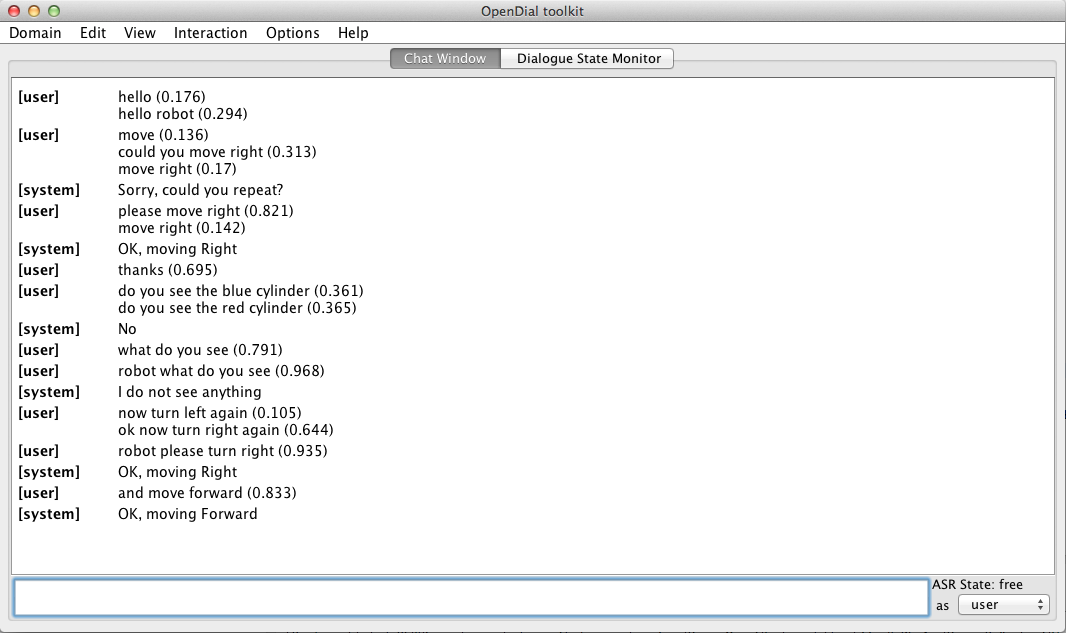
\includegraphics[scale=0.40]{imgs/gui-chatbox.png}
\caption{Graphical user interface showing the interaction history.}
\label{fig:gui-chatbox}
\end{figure}

  The user inputs are displayed as N-best lists together with their corresponding probabilities. In addition to monitoring the interaction, the chat window can also be used to test the dialogue system by typing new user and system inputs in the input field at the bottom of the window.  A drop-down field in the bottom right corner is used to switch the agent role (e.g.\ for Wizard-of-Oz experiments). 


\subsubsection*{Dialogue state monitor}
\index{dialogue state monitor}

To allow the system designer to easily inspect the content of the dialogue state, a state visualisation tool has also been integrated into \opendial{}.  The monitor provides a visual representation of the dialogue state in the form of a directed graph with nodes corresponding to the state variables and directed edges corresponding to conditional dependencies.\footnote{The graphs are rendered with JUNG, an open source toolkit for drawing graphs: \begin{scriptsize}\url{http://jung.sourceforge.net}\end{scriptsize}.} An example of a graph layout is shown in Figure \ref{fig:gui-bn}. The graph is dynamically refreshed after each update of the dialogue state, using graph drawing algorithms to optimise the layout of nodes on the screen. 

In addition to depicting the current dialogue state, the monitor also records and stores previous dialogue states.  The dialogue state to visualise can be selected among the list on the left side of the window. This functionality is particularly useful to compare dialogue states with one another and analyse how the dialogue state is evolving over time. 

\begin{figure}[p!] 
\begin{center}
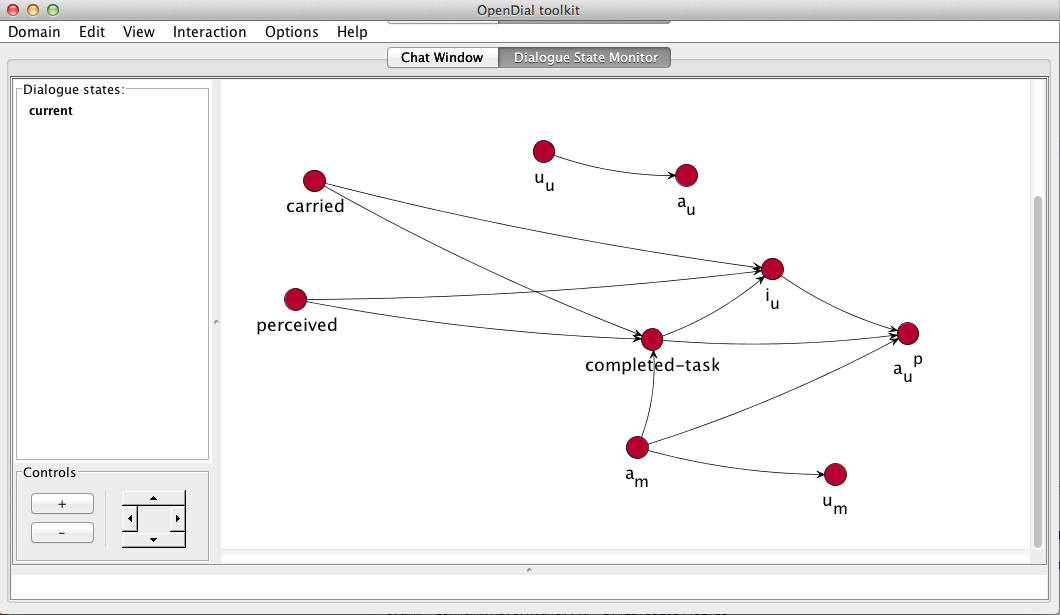
\includegraphics[scale=0.40]{imgs/gui-bn.png}
\end{center} 
\caption{Visualisation of the current dialogue state.}
\label{fig:gui-bn}
\end{figure}

\begin{figure}[p!] 
\begin{center}
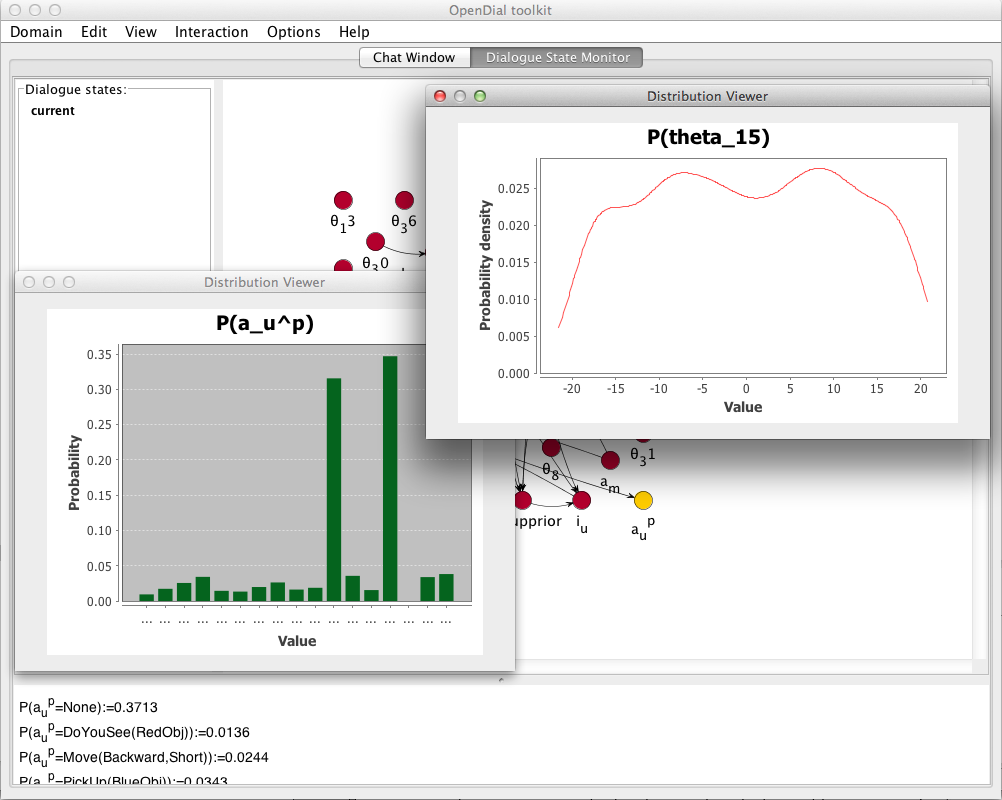
\includegraphics[scale=0.40]{imgs/gui-distribviewer.png}
\end{center} 
\caption{Visualisation of a discrete probability distribution $P(a_u^p)$ and a continuous probability distribution $P(\theta_{15})$ in the dialogue state monitor.}
\label{fig:gui-distribviewer}
\end{figure}

The user can manipulate the graph in multiple ways in order to e.g.\ analyse the content of specific state variables, add or remove evidence, or request the calculation of marginal distributions on a selected set of variables.  The inference results are in this case shown in the text area at the bottom of the window.  In addition, the system designer can also zoom in on selected probability distributions using the distribution viewer tool illustrated in Figure \ref{fig:gui-distribviewer}. Discrete probability distributions are shown as histograms, while continuous probability distributions are represented by their probability density functions.\footnote{The probability distributions are rendered with the open source toolkit JFreeChart: \begin{scriptsize}\url{http://jfreechart.sourceforge.net}\end{scriptsize}.} 


\section{Conclusion}

This chapter exposed the practical integration of our structured modelling framework in the \opendial{} toolkit and its instantiation in a spoken dialogue system for human--robot interaction. The first section presented the general architecture of the toolkit, the declarative specification of dialogue domains in an XML format, and the implementation of efficient algorithms for inference, sampling and planning. We discussed the benefits of using a shared description formalism in terms of transparency, portability, flexibility and adaptivity over traditional ``black-box'' architectures. We also compared \opendial{} to other existing architectures and pointed out a number of limitations in the current implementation of the toolkit, such as its lack of incremental processing and its limited turn-taking behaviour. 

The \opendial{} toolkit is inspired by both symbolic and statistical approaches to dialogue, and combines an information state architecture with probabilistic reasoning based on rule-structured models.  As stated in the introduction chapter, the long-term goal of the \opendial{} framework is to bridge the gap between symbolic approaches to dialogue management, which usually concentrate on capturing rich interaction patterns, and probabilistic approaches, more focused on aspects related to noise, uncertainty, and adaptivity. 

The hybrid design  of \opendial{} allows system designers to exploit powerful generalisations in the dialogue domain specification without sacrificing the probabilistic nature of the model. Another important side benefit of probabilistic rules is their improved readability for human experts, which are able to leverage their domain knowledge in the form of pragmatic rules, common sense assumptions, or task-specific constraints. Furthermore, the internal organisation of rules into models enables dialogue domains to be specified in a modular fashion, by clustering rules into distinct models.  Some models may therefore reflect highly domain-specific knowledge while others encode generic interaction patterns that can easily be ported to other applications.  

The last section described the integrated dialogue system used to carry out the practical experiments presented in Chapters \ref{chap:wozlearning}, \ref{chap:rllearning} and \ref{chap:user-evaluation}.  The system comprised both synchronous and asynchronous components and included dedicated modules for speech recognition, speech synthesis, robot perception and motor control.  Natural language understanding, dialogue management and natural language generation were encoded with models structured with probability rules. 

The next chapter demonstrates the practical deployment of this system in a full-scale user evaluation study. 